\documentclass[10pt]{article}

\usepackage{graphicx}
\usepackage{amsmath}
%\usepackage[ansinew]{inputenc}
\usepackage[utf8]{inputenc}
\usepackage[spanish]{babel}
\usepackage{babelbib}
\usepackage[T1]{fontenc}
\usepackage[vmargin=4cm,hmargin=4cm,letterpaper]{geometry}
\usepackage{color}
\usepackage{framed}
\usepackage{hyperref}

\usepackage{listings}
\definecolor{red}{RGB}{219,0,0}
\definecolor{pink}{RGB}{255,100,100}
\definecolor{gray}{RGB}{100,100,100}
\lstset{
		basicstyle=\tiny,
		frame=single,
		keywordstyle=\color{red},
		commentstyle=\color{gray},
		stringstyle=\color{pink},
		tabsize=3,
		language=verilog,
		backgroundcolor=\color{white}}

\usepackage{fancyhdr} 
\pagestyle{fancy}
\usepackage{lastpage}
\lhead{Laboratorio 3}
\chead{}
\rhead{Bitácora}
\lfoot{}
\cfoot{}
\rfoot{\footnotesize Page \thepage\ of \pageref{LastPage}}

\renewcommand{\headrulewidth}{0.4pt} 
\renewcommand{\footrulewidth}{0.4pt} 

\graphicspath{{images/}}	%%multimedia path
\setlength{\parindent}{0pt}
%%*************************************************************************
\begin{document}

\begin{huge}
\begin{center}
\textbf{Laboratorio 3: Circuitos combinatorios}
\end{center}
\end{huge}

\begin{Large}
\begin{center}
Jose Apú (B10407), Francisco Molina (B14194), \\Marco Montero (A94000), Dennis Vargas (B16831)
\end{center}
\end{Large}


\section*{Ejercicio 1}
Implemente una máquina de estados en el Spartan 6 que cumpla con la temporización necesaria para escribir y leer datos de una memoria SRAM en una plataforma Papilio Duo.\\[0.3 cm]

Para este ejercicio se instanció en la MiniAlu del Spartan 6 el controlador de una SRAM creado a partir de una máquina de estados encargada de manejar las diferentes señales necesarias en los diferentes pines para el correcto funcionamiento de escritura y lectura sobre la SRAM. Posterior a esto se escribió una serie de instrucciones en la MiniAlu de forma que la escritura y la lectura a las diferentes posiciones de la memoria fuera transparente para el usuario. Por último se escribió en la ROM un programa de prueba que escribiera y leyera datos en la memoria y escribiera los ultimos 8 bits en los LEDs de la Papilio Duo. El Papilio duo, tiene una fpga, un wing que permite usar leds para ver que está leyendo y escribiendo, esto funciona para debuggear. \\



\begin{figure}[hbtp]
\centering
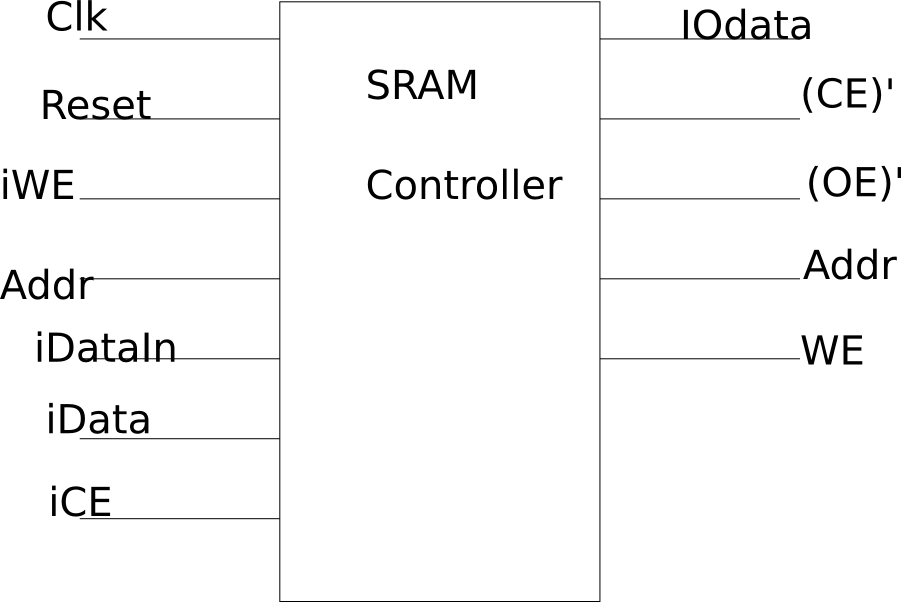
\includegraphics[width=10cm]{sramcontroller.png}
\caption{Diagrama Controlador SRAM}
\label{Con1}
\end{figure}

Además la tabla de verdad para este controlador será la siguiente:

\begin{figure}[hbtp]
\centering
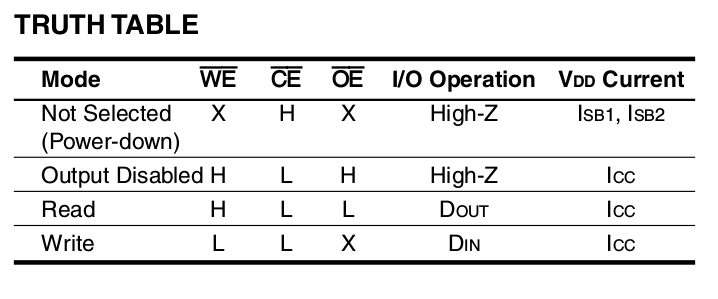
\includegraphics[width=10cm]{truth-table.png}
\caption{Tabla de verdad}
\label{tab1}
\end{figure}

\newpage

\subsection*{Temporización}

Para el correcto funcionamiento del controlador, el mismo debe cumplir con ciertos tiempos establecidos por el fabricante de la SRAM que está contenida en el papillio duo. El cumplimiento de estos tiempos llevará a que se pueda escribir o leer correctamente sobre la SRAM.
Cabe destacar que los tiempos a cumplir para el ciclo de escritura y lectura son distintos.

\begin{figure}[hbtp]
\centering
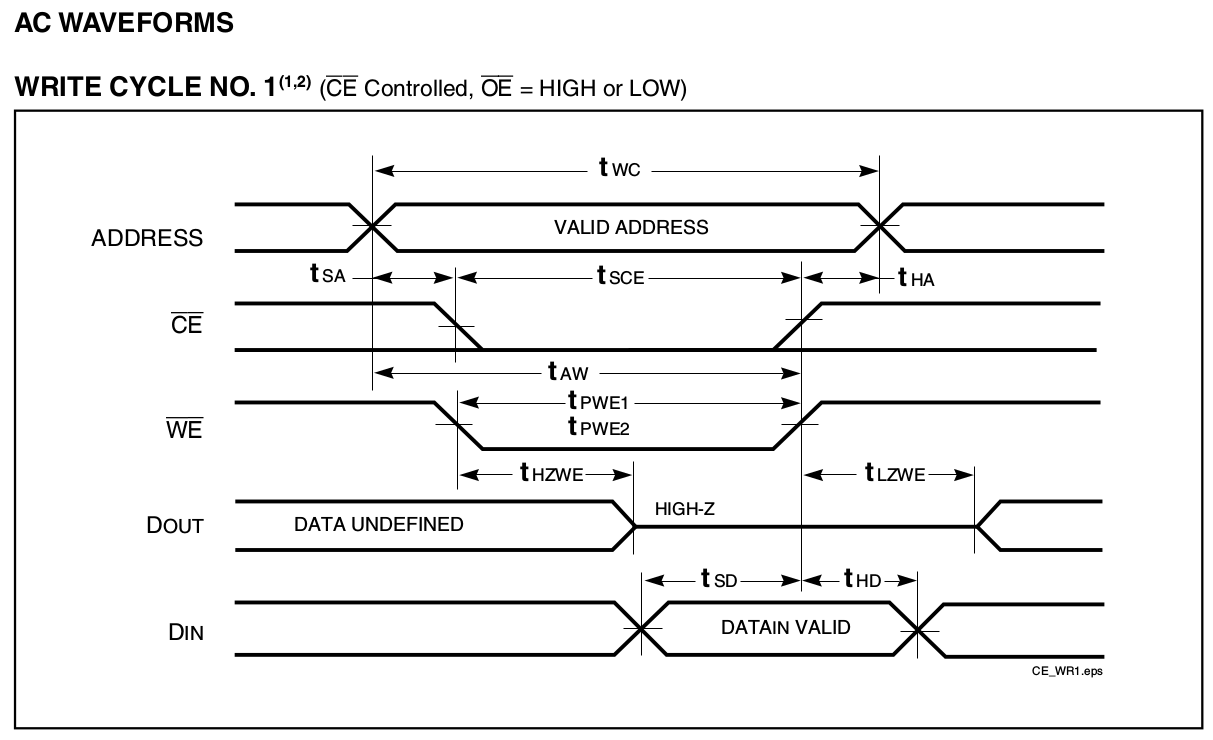
\includegraphics[width=10cm]{write-form.png}
\caption{Ciclo escritura}
\label{Cic1}
\end{figure}

\begin{figure}[hbtp]
\centering
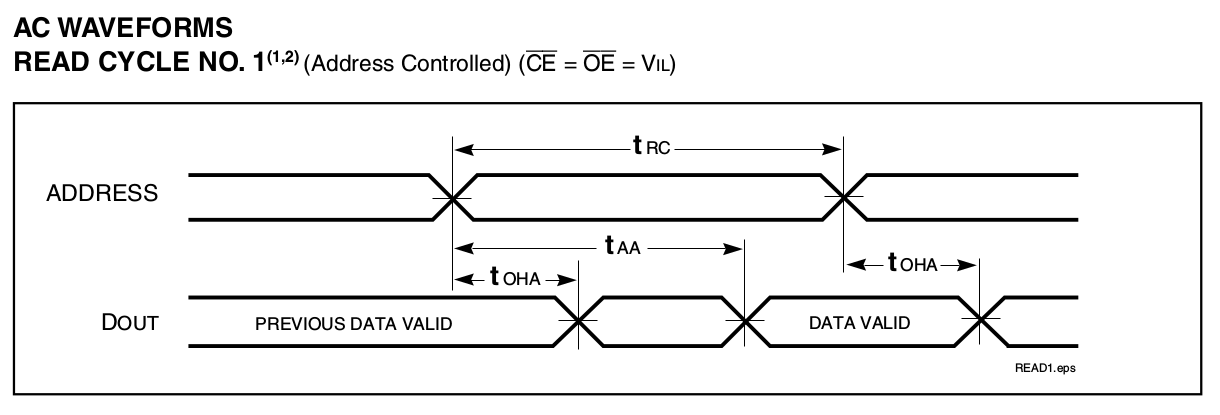
\includegraphics[width=10cm]{read-form.png}
\caption{Ciclo lectura}
\label{Cic2}
\end{figure}

\newpage

Además para nuestro trabajo la papillio esta definida para ciclos de trabajo de un rango de 20ns. Por lo tanto los tiempos min y max a cumplir son los correspodientes a la columna $"$-20ns$"$ en las tablas siguientes:

\begin{figure}[hbtp]
\centering
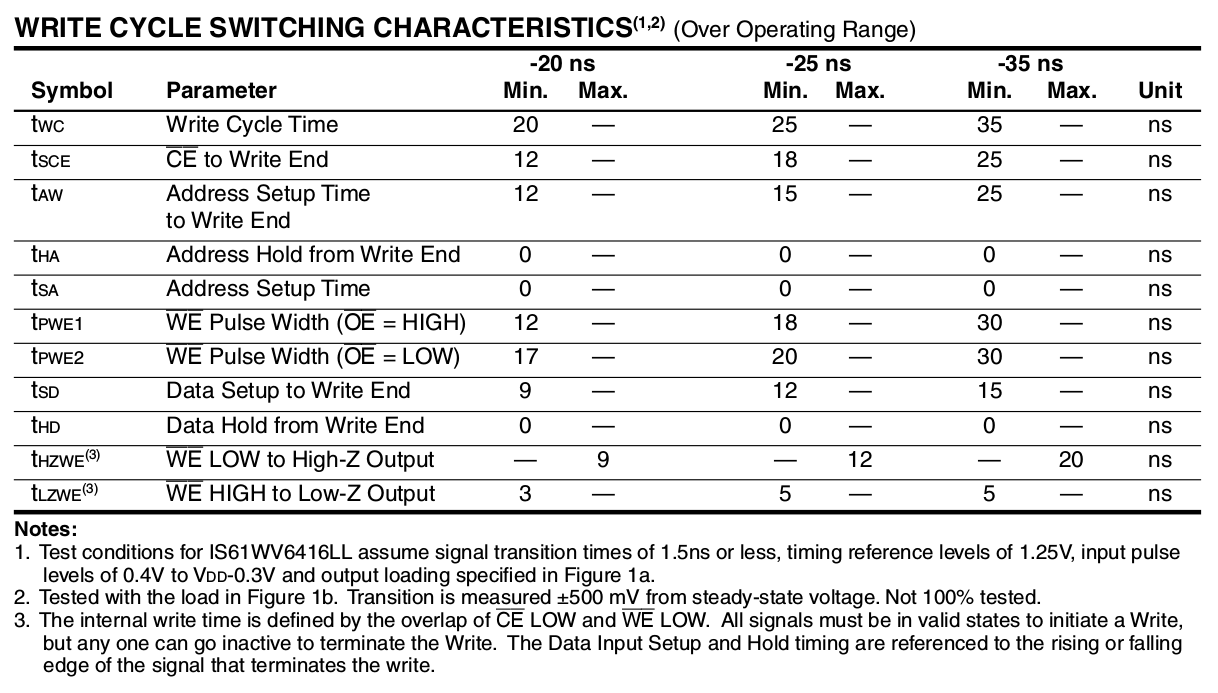
\includegraphics[width=10cm]{write-data.png}
\caption{Ciclo escritura}
\label{Cic3}
\end{figure}

\begin{figure}[hbtp]
\centering
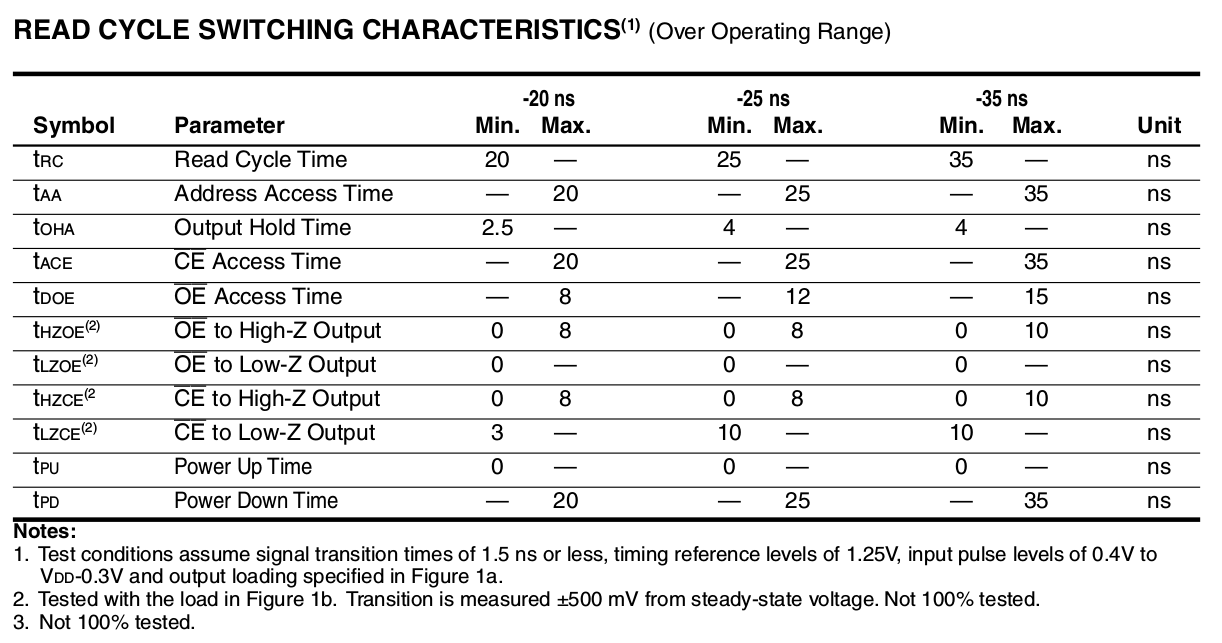
\includegraphics[width=10cm]{read-data.png}
\caption{Ciclo lectura}
\label{Cic4}
\end{figure}

\newpage


\subsection*{SRAM controller}
\begin{lstlisting}
`define LISTEN 		  0
`define WRITE_SETUP   1
`define WRITE 		  2
`define WRITE_HOLD 	  3
`define READ_REQUEST  4
`define READ_LATCH    5


// SPARTAN 6
// CoreSpeed 32Mhz
// SRAM writting times 
// tSA  = 4ns;
// tSCE = 12ns;
// tHA  = 4ns;
// SRAM reading times
// tRC = 20ns

module SRAM_CONTROLLER # ( parameter DATA_WIDTH= 8, parameter ADDR_WIDTH=19 )
(
	input wire							Clock,
	input wire							Reset,
	
	//R/W Selection
	input wire 							iWriteEnable,	     
	//Enable the SRAM R/W
	input wire 							iTrigger,		     
	//Data from MiAlu
	input wire [ADDR_WIDTH-1:0]		iAddress,           
	//Data that the guest wants to write into SRAM
	input wire [DATA_WIDTH-1:0] 		iDataIn,            
	//Data from SRAM
	input wire [DATA_WIDTH-1:0]		iSRAMDataIn,        
	//Data that was read from SRAM
	output wire [DATA_WIDTH-1:0]		oSRAMDataRead,      
	//Data that we want to write into SRAM
	output wire [DATA_WIDTH-1:0] 		oSRAMDataWrite,     
	//Address to read/write to SRAM
	output wire [ADDR_WIDTH-1:0]		oSRAMAddressOut,     
	output reg                      oSRaMWriteEnable
);

reg wAddrEn, rDataWriteHold ;
reg rDataReadEn, rDataWriteEn;
wire [DATA_WIDTH-1:0] wSRAMDataWrite;


assign oSRAMDataWrite = ( rDataWriteEn ) ?  wSRAMDataWrite : 8'bz ;


FFD_POSEDGE_SYNCRONOUS_RESET # ( ADDR_WIDTH ) FFD_ADDR 
(
	.Clock(  Clock        ),
	.Reset(  Reset        ),
	.Enable( wAddrEn      ),
	.D(      iAddress     ),
	.Q(      oSRAMAddressOut  )
);


FFD_POSEDGE_SYNCRONOUS_RESET # ( DATA_WIDTH ) FFD_DATAOUT 
(
	.Clock(  Clock           ),
	.Reset(  Reset           ),
	.Enable( rDataWriteHold  ),
	.D(      iDataIn         ),
	.Q(      wSRAMDataWrite  )
);


FFD_POSEDGE_SYNCRONOUS_RESET # ( DATA_WIDTH ) FFD_DATAIN 
(
	.Clock(  Clock            ),
	.Reset(  Reset            ),
	.Enable( rDataReadEn      ),
	.D(      iSRAMDataIn      ),
	.Q(      oSRAMDataRead    )
);

reg [3:0] rCurrentState, rNextState;
reg [ADDR_WIDTH-1:0]    rNextAddr;
reg [DATA_WIDTH-1:0]    rNextDataOut;

//Logica de Estado Presente
always @ ( posedge Clock, posedge Reset )
begin
	if (Reset)
		rCurrentState <= `LISTEN;
	else
		rCurrentState <= rNextState;
end

//Logica de Proximo Estado de una Maquina de Mealy
always @ ( * )
begin
	case (rCurrentState)

		`LISTEN:
		begin
			//Hold address in this state to make sure it`ll be available in next state
			wAddrEn  = 1'b1;	
			rDataReadEn  = 1'b0;
			rDataWriteEn = 1'b0;
			rDataWriteHold = iWriteEnable;
			oSRaMWriteEnable = 1'b1;

			if (iTrigger)
				   rNextState = ( iWriteEnable ) ? `WRITE_SETUP : `READ_REQUEST  ;
			else 
			      rNextState = `LISTEN;
		end

		`WRITE_SETUP:
		begin
			wAddrEn          = 1'b0;
			rDataReadEn      = 1'b0;
			rDataWriteEn     = 1'b0;
			rDataWriteHold   = 1'b0;
			oSRaMWriteEnable = 1'b1;

			rNextState = `WRITE;
			
		end

		`WRITE:
		begin
			wAddrEn          = 1'b0;
			rDataReadEn      = 1'b0;
			rDataWriteEn     = 1'b0;
			rDataWriteHold   = 1'b0;
			oSRaMWriteEnable = 1'b1;
NET "oSramAddr<0>" LOC = "P7" | IOSTANDARD=LVTTL | SLEW=FAST;
NET "oSramAddr<1>" LOC = "P8" | IOSTANDARD=LVTTL | SLEW=FAST ;
NET "oSramAddr<2>" LOC = "P9" | IOSTANDARD=LVTTL | SLEW=FAST ;
NET "oSramAddr<3>" LOC = "P10" | IOSTANDARD=LVTTL | SLEW=FAST ;
NET "oSramAddr<4>" LOC = "P11" | IOSTANDARD=LVTTL | SLEW=FAST ;
NET "oSramAddr<5>" LOC = "P5" | IOSTANDARD=LVTTL | SLEW=FAST ;
NET "oSramAddr<6>" LOC = "P2" | IOSTANDARD=LVTTL | SLEW=FAST ;
NET "oSramAddr<7>" LOC = "P1" | IOSTANDARD=LVTTL | SLEW=FAST ;
NET "oSramAddr<8>" LOC = "P143" | IOSTANDARD=LVTTL | SLEW=FAST ;
NET "oSramAddr<9>" LOC = "P142" | IOSTANDARD=LVTTL | SLEW=FAST ;
NET "oSramAddr<10>" LOC = "P43" | IOSTANDARD=LVTTL | SLEW=FAST ;
NET "oSramAddr<11>" LOC = "P41" | IOSTANDARD=LVTTL | SLEW=FAST ;
NET "oSramAddr<12>" LOC = "P40" | IOSTANDARD=LVTTL | SLEW=FAST;
NET "oSramAddr<13>" LOC = "P35" | IOSTANDARD=LVTTL | SLEW=FAST ;
NET "oSramAddr<14>" LOC = "P34" | IOSTANDARD=LVTTL | SLEW=FAST ;
NET "oSramAddr<15>" LOC = "P27" | IOSTANDARD=LVTTL | SLEW=FAST ;
NET "oSramAddr<16>" LOC = "P29" | IOSTANDARD=LVTTL | SLEW=FAST ;
NET "oSramAddr<17>" LOC = "P33" | IOSTANDARD=LVTTL | SLEW=FAST ;
NET "oSramAddr<18>" LOC = "P32" | IOSTANDARD=LVTTL | SLEW=FAST ;
#NET "oSramAddr<19>" LOC = "P44" | IOSTANDARD=LVTTL | SLEW=FAST ;
#NET "oSramAddr<20>" LOC = "P30" | IOSTANDARD=LVTTL | SLEW=FAST ;
NET "oSramData<0>" LOC = "P14" | IOSTANDARD=LVTTL | SLEW=FAST ;
NET "oSramData<1>" LOC = "P15" | IOSTANDARD=LVTTL | SLEW=FAST ;
NET "oSramData<2>" LOC = "P16" | IOSTANDARD=LVTTL | SLEW=FAST ;
NET "oSramData<3>" LOC = "P17" | IOSTANDARD=LVTTL | SLEW=FAST ;
NET "oSramData<4>" LOC = "P21" | IOSTANDARD=LVTTL | SLEW=FAST ;
NET "oSramData<5>" LOC = "P22" | IOSTANDARD=LVTTL | SLEW=FAST ;
NET "oSramData<6>" LOC = "P23" | IOSTANDARD=LVTTL | SLEW=FAST ;
NET "oSramData<7>" LOC = "P24" | IOSTANDARD=LVTTL | SLEW=FAST ;
NET "oSramCe" LOC = "P12" | IOSTANDARD=LVTTL | SLEW=FAST;
NET "oSramWe" LOC = "P6" | IOSTANDARD=LVTTL | SLEW=FAST ;
NET "oSramOe" LOC = "P26" | IOSTANDARD=LVTTL | SLEW=FAST
			rNextState = `WRITE_HOLD;
		end

		`WRITE_HOLD:
		begin
			wAddrEn          = 1'b0;
			rDataReadEn      = 1'b0;
			rDataWriteEn     = 1'b1;
			rDataWriteHold   = 1'b0;
			oSRaMWriteEnable = 1'b0;

			rNextState = `LISTEN;
		end

		`READ_REQUEST:			//Present address bus
		begin	
			wAddrEn          = 1'b0;
			rDataReadEn      = 1'b0;
			rDataWriteEn     = 1'b0;
			rDataWriteHold   = 1'b0;
			oSRaMWriteEnable = 1'b1;

			rNextState = `READ_LATCH;
		end

		`READ_LATCH:           //Readback data from Memory
		begin
			wAddrEn          = 1'b0;
         rDataReadEn      = 1'b1;
         rDataWriteEn     = 1'b0;
			rDataWriteHold   = 1'b0;
			oSRaMWriteEnable = 1'b1;

			rNextState = `LISTEN;
		end


		default:
		begin
			wAddrEn          =  1'b0;
			rDataReadEn      =  1'b0;
			rDataWriteEn     = 1'b0;
			rDataWriteHold   = 1'b0;
			oSRaMWriteEnable = 1'b1;

			rNextState = `LISTEN;
		end

	endcase
end

endmodule
\end{lstlisting}


\subsection*{Pines y conexión física}

Por último para poder poner en funcionamiento el controlador se debe definir los pines que comunican la FPGA con la SRAM, esto para poder realizar la conexión física entre ambos, de esta manera las salidas que levante el SRAMController creado, tendrán un sentido físico.
Esto se logra modificando el archivo minualu\_logic\_start\_mega\_wing.ucf añadiendo la siguiente información relevante:


\begin{lstlisting}
NET "oSramAddr<0>" LOC = "P7" | IOSTANDARD=LVTTL | SLEW=FAST;
NET "oSramAddr<1>" LOC = "P8" | IOSTANDARD=LVTTL | SLEW=FAST ;
NET "oSramAddr<2>" LOC = "P9" | IOSTANDARD=LVTTL | SLEW=FAST ;
NET "oSramAddr<3>" LOC = "P10" | IOSTANDARD=LVTTL | SLEW=FAST ;
NET "oSramAddr<4>" LOC = "P11" | IOSTANDARD=LVTTL | SLEW=FAST ;
NET "oSramAddr<5>" LOC = "P5" | IOSTANDARD=LVTTL | SLEW=FAST ;
NET "oSramAddr<6>" LOC = "P2" | IOSTANDARD=LVTTL | SLEW=FAST ;
NET "oSramAddr<7>" LOC = "P1" | IOSTANDARD=LVTTL | SLEW=FAST ;
NET "oSramAddr<8>" LOC = "P143" | IOSTANDARD=LVTTL | SLEW=FAST ;
NET "oSramAddr<9>" LOC = "P142" | IOSTANDARD=LVTTL | SLEW=FAST ;
NET "oSramAddr<10>" LOC = "P43" | IOSTANDARD=LVTTL | SLEW=FAST ;
NET "oSramAddr<11>" LOC = "P41" | IOSTANDARD=LVTTL | SLEW=FAST ;
NET "oSramAddr<12>" LOC = "P40" | IOSTANDARD=LVTTL | SLEW=FAST;
NET "oSramAddr<13>" LOC = "P35" | IOSTANDARD=LVTTL | SLEW=FAST ;
NET "oSramAddr<14>" LOC = "P34" | IOSTANDARD=LVTTL | SLEW=FAST ;
NET "oSramAddr<15>" LOC = "P27" | IOSTANDARD=LVTTL | SLEW=FAST ;
NET "oSramAddr<16>" LOC = "P29" | IOSTANDARD=LVTTL | SLEW=FAST ;
NET "oSramAddr<17>" LOC = "P33" | IOSTANDARD=LVTTL | SLEW=FAST ;
NET "oSramAddr<18>" LOC = "P32" | IOSTANDARD=LVTTL | SLEW=FAST ;
#NET "oSramAddr<19>" LOC = "P44" | IOSTANDARD=LVTTL | SLEW=FAST ;
#NET "oSramAddr<20>" LOC = "P30" | IOSTANDARD=LVTTL | SLEW=FAST ;
NET "oSramData<0>" LOC = "P14" | IOSTANDARD=LVTTL | SLEW=FAST ;
NET "oSramData<1>" LOC = "P15" | IOSTANDARD=LVTTL | SLEW=FAST ;
NET "oSramData<2>" LOC = "P16" | IOSTANDARD=LVTTL | SLEW=FAST ;
NET "oSramData<3>" LOC = "P17" | IOSTANDARD=LVTTL | SLEW=FAST ;
NET "oSramData<4>" LOC = "P21" | IOSTANDARD=LVTTL | SLEW=FAST ;
NET "oSramData<5>" LOC = "P22" | IOSTANDARD=LVTTL | SLEW=FAST ;
NET "oSramData<6>" LOC = "P23" | IOSTANDARD=LVTTL | SLEW=FAST ;
NET "oSramData<7>" LOC = "P24" | IOSTANDARD=LVTTL | SLEW=FAST ;
NET "oSramCe" LOC = "P12" | IOSTANDARD=LVTTL | SLEW=FAST;
NET "oSramWe" LOC = "P6" | IOSTANDARD=LVTTL | SLEW=FAST ;
NET "oSramOe" LOC = "P26" | IOSTANDARD=LVTTL | SLEW=FAST
\end{lstlisting}

%%**********************************************************************
\section{Prueba}
Primero se escriben los datos en la SRAM. Para lograrlo, se escribe en la ROM lo siguiente:

\begin{lstlisting}
...
4: oInstruction = { `STO , `R4, 8'b0, 8'b11010100};
5: oInstruction = { `STO , `R5, 8'b0, 8'b11101000};
...
7: oInstruction = { `SWR , 8'hff, `R4, `R1};
...
11: oInstruction = { `SWR , 8'hff, `R5, `R2};
...
\end{lstlisting}

En la simulación se observa como se escriben los datos escritos, ver Figura \ref{sim_escritura}

% Adding an image
\begin{figure}[hbtp]
\centering
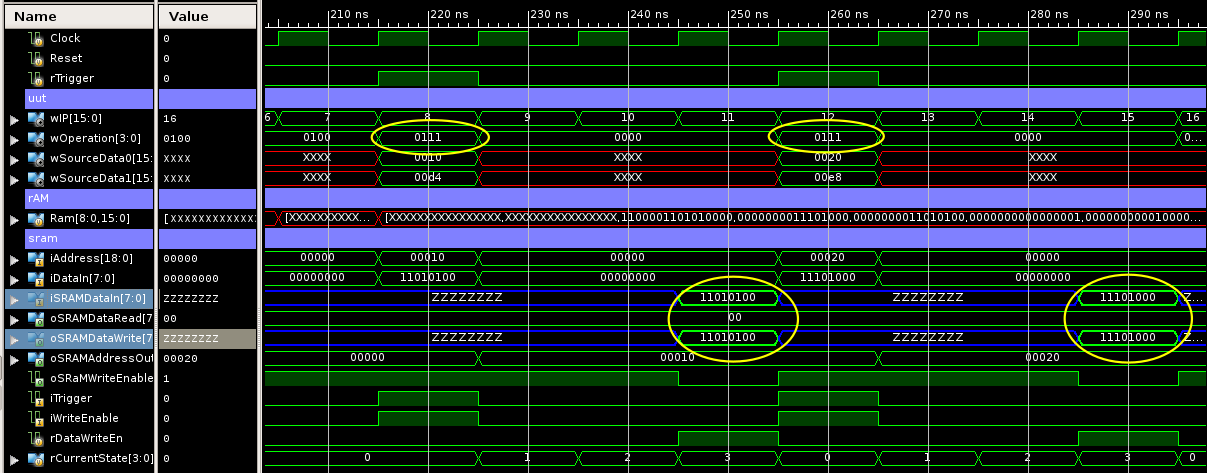
\includegraphics[width=1\textwidth]{escritura.png}
\caption{Simulación: Escritura}
\label{sim_escritura}
\end{figure}

Para leerlos se utilizan los leds. Para lograrlo, se escribe en la ROM lo siguiente:

\begin{lstlisting}
...
17: oInstruction = { `SRD , `R4, 8'hff, `R1};
...
21: oInstruction = { `LED , 8'hff, 8'hff, `R4 };
...
28: oInstruction = { `SRD , `R5, 8'hff, `R2};
...
32: oInstruction = { `LED , 8'hff, 8'hff, `R5 };
...
\end{lstlisting}

En las fotografías se observan como los leds ilustran los dos datos escritos y a su vez leidos. Ver Figuras \ref{lectura_1} y \ref{lectura_2}

% Adding an image
\begin{figure}[hbtp]
\centering
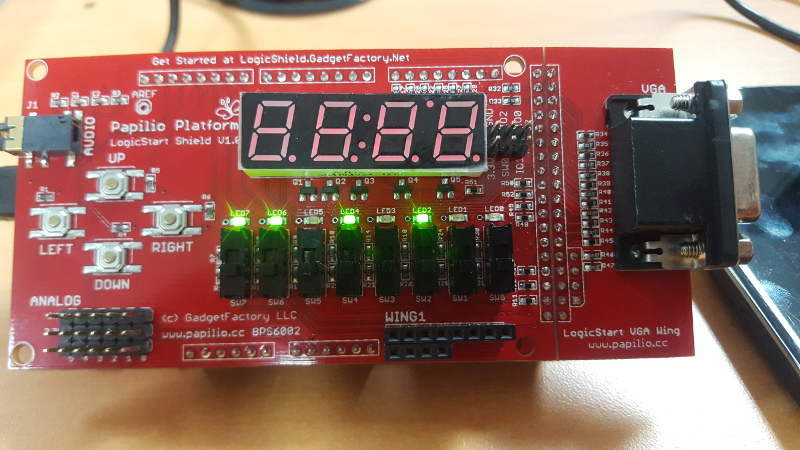
\includegraphics[width=1\textwidth]{lecturaa.jpg}
\caption{Lectura del primer dato}
\label{lectura_1}
\end{figure}

% Adding an image
\begin{figure}[hbtp]
\centering
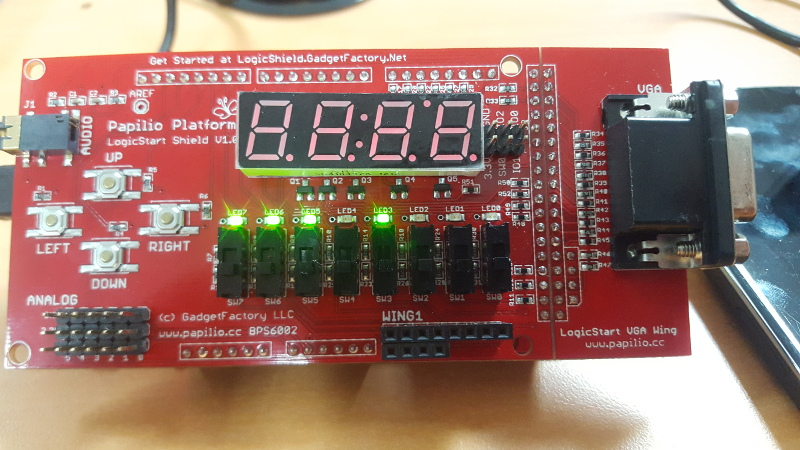
\includegraphics[width=1\textwidth]{lecturab.jpg}
\caption{Lectura del segundo dato}
\label{lectura_2}
\end{figure}
\pagebreak
%%**********************************************************************
\section{Conlusiones}
Se logra crear un controlador para la SRAM apartir de una máquina de estados, gracias al mismo se puede establecer una comunicación entre la SRAM y la FPGA SPARTAN6 que permite escribir o leer posiciones de está memoria estática. Cabe destacar que además el controlador utilizó el diagrama de pines para lograr esa comunicación física entre ambos.\\
%%**********************************************************************
\section{Bibliografía}
\begin{itemize}
\item Información Papillio Duo.http://papilio.cc/index.php?n=Papilio.PapilioDUOHardwareGuide
\item Archivos .v descargados del drive del profesor Diego Valverde.
\end{itemize}

\end{document}
%%*************************************************************************
